\documentclass{scrartcl}
\usepackage[utf8]{inputenc}
\usepackage{hyperref}
\usepackage{url}
\usepackage{natbib}
\usepackage{graphicx}
\usepackage{listings}

\newcommand{\emailaddr}[1]{\href{mailto:#1}{\texttt{#1}}}

\title{\LARGE
    CityTwin
}

% Consider watching:
% https://www.youtube.com/watch?v=ihxSUsJB_14
% https://www.youtube.com/watch?v=XTFWaV55uDo

\author{
    Filippo Vissani \\ \emailaddr{filippo.vissani@studio.unibo.it}
    \and 
    Eddie Barzi \\ \emailaddr{eddie.barzi@studio.unibo.it}
}

\date{September 2023}

\begin{document}

\maketitle

\begin{abstract}
    %Up to $\sim$2000 characters briefly describing the project.

    Il progetto CityTwin si propone di realizzare la simulazione di un sistema di digital twin nel contesto della smart city. In particolare, si vuole realizzare un sistema che sia in grado di catturare e rappresentare in formato digitale il comportamento delle varie entità presenti all'interno della città. Questo può portare ad una serie di benefici, alcuni dei quali vengono elencati di seguito:

    \begin{itemize}
        \item Rilevazione di possibili problematiche con intervento tempestivo e automatizzato.
        \item Riduzione del consumo energetico.
        \item Rilevazione della qualità dell'aria e dell'acqua.
        \item Analisi dell'inquinamento acustico.
        \item Ottimizzazione della mobilità urbana.
    \end{itemize}

    La simulazione sarà composta da due tipologie di nodi: i nodi Mainstay, che rappresentano la struttura portante del sistema, e i nodi Resource, che rappresentano astrazioni di sensori, attuatori o entità più complesse.

    I nodi Mainstay si occupano di scambiare informazioni con i nodi Resource, rilevare eventuali malfunzionamenti e salvare in modo persistente le informazioni rilevate dai nodi Resource. I nodi Mainstay devono essere sempre sincronizzati tra loro, in modo da poter garantire la coerenza dei dati.

    I nodi Resource, invece, si occupano di rilevare informazioni e comunicarle ai nodi Mainstay nel caso in cui vengano considerati come sensori. Nel caso in cui i nodi Resource rappresentino attuatori, invece, si occupano di ricevere informazioni dai nodi Mainstay e agire di conseguenza.

    Per la memorizzazione delle dello stato dei nodi viene disposto un servizio apposito di persistenza dei dati. Tale servizio viene utilizzato sia dai nodi Mainstay che da altri clienti, come ad esempio il pannello di controllo.

    L'utente potrà visualizzare lo stato attuale del sistema, lo storico dei dati ed eventuali statistiche, nonché interagire con il sistema tramite GUI, ad esempio per intervenire dopo la rilevazione di un incendio.

\end{abstract}

\section{Goal/Requirements}

Detailed description of the project goals, requirements, and expected outcomes.
%
Use case Diagrams, examples, or Q/A simulations are welcome.

\subsection{Scenarios}

Informal description of the ways users are expected to interact with your project.
%
It should describe \emph{how} and \emph{why} a user should use / interact with the system.

\subsection{Self-assessment policy}

\begin{itemize}
    \item How should the \emph{quality} of the \emph{produced software} be assessed?

    \item How should the \emph{effectiveness} of the project outcomes be assessed?
\end{itemize}

\section{Requirements Analysis}

Is there any implicit requirement hidden within this project's requirements?
%
Is there any implicit hypothesis hidden within this project's requirements?
%
Are there any non-functional requirements implied by this project's requirements?

What model / paradigm / techonology is the best suited to face this project's requirements?
%
What's the abstraction gap among the available models / paradigms / techonologies and the problem to be solved?

\section{Progettazione}

\subsection{Architettura del Sistema}

L'architettura del sistema, presentata in Figura \ref{fig:core-component-diagram}, è organizzata intorno a componenti interconnessi che consentono il monitoraggio e la gestione delle entità presenti all'interno della città. Ogni componente svolge ruoli specifici all'interno del sistema e interagisce attraverso interfacce ben definite.

In Figura \ref{fig:nodes-component-diagram} viene presentata l'architettura dei componenti in esecuzione e dei protocolli di rete utilizzati. Il sistema è costituito da un insieme di nodi \textit{Mainstay} e \textit{Resource} che comunicano tra loro attraverso il protocollo \textit{Akka}. Inoltre, i nodi \textit{Mainstay} comunicano con il servizio di persistenza attraverso il protocollo \textit{HTTP}.
I nodi che comunicano utilizzando il protocollo \textit{Akka} sono \textit{Actor System} organizzati in un cluster, in modo da poter garantire la scalabilità del sistema.

\subsubsection{Core}
Il componente centrale del sistema è il \textit{Core}, responsabile della gestione dell'elaborazione dati, del coordinamento delle attività e della comunicazione tra gli altri componenti. Il Core funge da mediatore tra le varie risorse presenti all'interno della città, ricevendo dati dai sensori e inviandoli al servizio di persistenza.

L'architettura del modulo \textit{Core} (Figura \ref{fig:core-class-diagram}) è costituita da diversi attori, ognuno dei quali svolge un ruolo specifico nel processo di acquisizione, gestione e comunicazione dei dati relativi alle risorse.

\textit{Resource Actor} è responsabile della gestione della risorsa, indipendentemente dal fatto che essa sia un sensore o un attuatore. Comunica con il \textit{Mainstay Actor} per ottenere o mandare lo stato delle risorse. È in grado di ricevere comandi e cambiamenti relativi alle risorse.

Il \textit{Mainstay Actor} si occupa di tenere in piedi l'intero sistema distribuito. Esso scambia lo stato delle risorse con il \textit{Resource Actor} e comunica con il \textit{Persistence Service Driver Actor} per salvare i dati nel servizio di persistenza. Inoltre, il \textit{Mainstay Actor} è responsabile della sincronizzazione dei nodi \textit{Mainstay}.

Il \textit{Nodes Observer Actor} monitora gli stati dei nodi all'interno del sistema e aggiorna il \textit{Mainstay Actor} sulla base del cambiamento di stato dei nodi.

L'attore \textit{Persistence Service Driver} è responsabile della gestione delle operazioni di persistenza dei dati. Comunica con il \textit{Mainstay Actor} per pubblicare nuovi dati al servizio di persistenza.

L'architettura prevede interazioni chiare e ben definite tra gli attori attraverso l'utilizzo di comandi specifici.

Il \textit{Resource Actor} comunica con il \textit{Mainstay Actor} utilizzando comandi come \textit{AskResourcesState}, \textit{AskAllResourcesState} e \textit{UpdateResources}. Queste interazioni consentono al \textit{Resource Actor} di ottenere informazioni sullo stato delle risorse e di aggiornare lo stato stesso.

Il \textit{Mainstay Actor} comunica con il \textit{Persistence Service Driver Actor} utilizzando comandi come \textit{PostMainstay} e \textit{PostResource}. Queste interazioni consentono al \textit{Mainstay Actor} di inviare nuovi dati al servizio di persistenza.

\begin{figure}[h]
    \caption{Diagramma delle classi del modulo \textit{Core}.}
    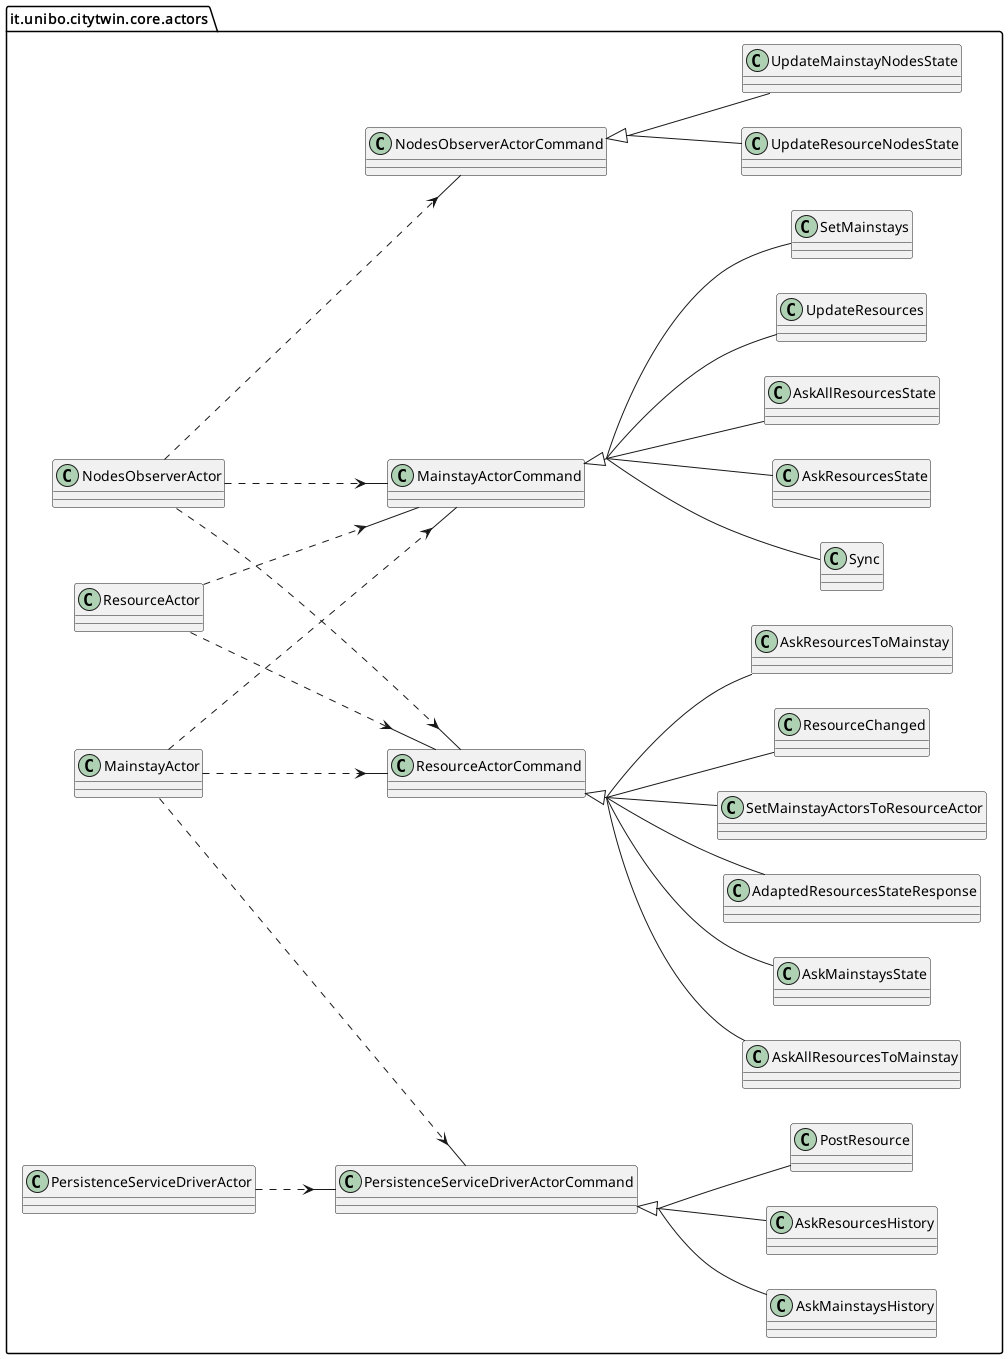
\includegraphics[width=\textwidth]{../assets/images/core-class-diagram.png}
    \label{fig:core-class-diagram}
\end{figure}

\subsubsection{Componenti Monitor}
I diversi monitor ambientali, come l'\textit{Acid Rain Monitor}, l'\textit{Air Quality Monitor}, il \textit{Noise Pollution Monitor} e il \textit{River Monitor}, costituiscono le fonti primarie di dati. Ciascun monitor raccoglie misurazioni specifiche e invia queste informazioni al \textit{Core} tramite l'interfaccia \textit{Resource}. Questa comunicazione consente al \textit{Core} di elaborare i dati e fornire una visione completa delle condizioni ambientali.

\subsubsection{Control Panel}
Il \textit{Control Panel} è l'interfaccia utente principale attraverso cui gli utenti interagiscono con il sistema. Comunica con il \textit{Core} per ottenere dati sullo stato ambientale e sul sistema nel suo complesso. Inoltre, il pannello di controllo richiede al servizio di persistenza lo storico dei dati in modo da poterli elaborare per ottenere delle statistiche.

\subsubsection{Persistence Service}
Il \textit{Persistence Service} gestisce la persistenza dei dati nel sistema. Comunica con il \textit{Core} attraverso le interfacce \textit{Post Resource} e \textit{Post Mainstay} per ricevere e salvare i dati relativi alle risorse. Analogamente, le interfacce \textit{Get Mainstay} e \textit{Get Resource }consentono di richiedere i dati al servizio di persistenza.

\begin{figure}[h]
    \caption{Diagramma dei componenti del sistema e delle loro dipendenze.}
    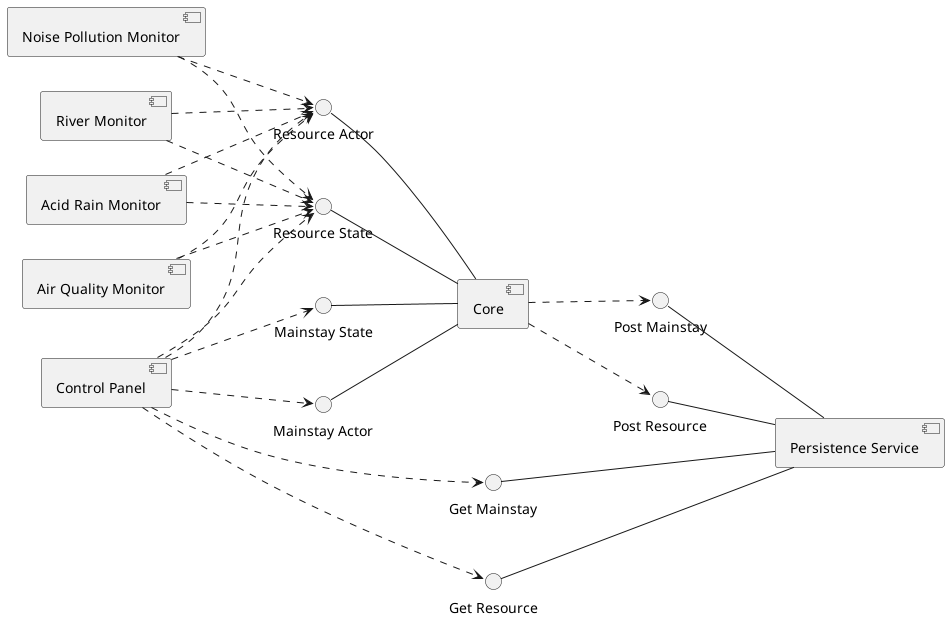
\includegraphics[width=\textwidth]{../assets/images/core-component-diagram.png}
    \label{fig:core-component-diagram}
\end{figure}

\begin{figure}[h]
    \caption{Diagramma dei componenti in esecuzione e dei protocolli di rete utilizzati.}
    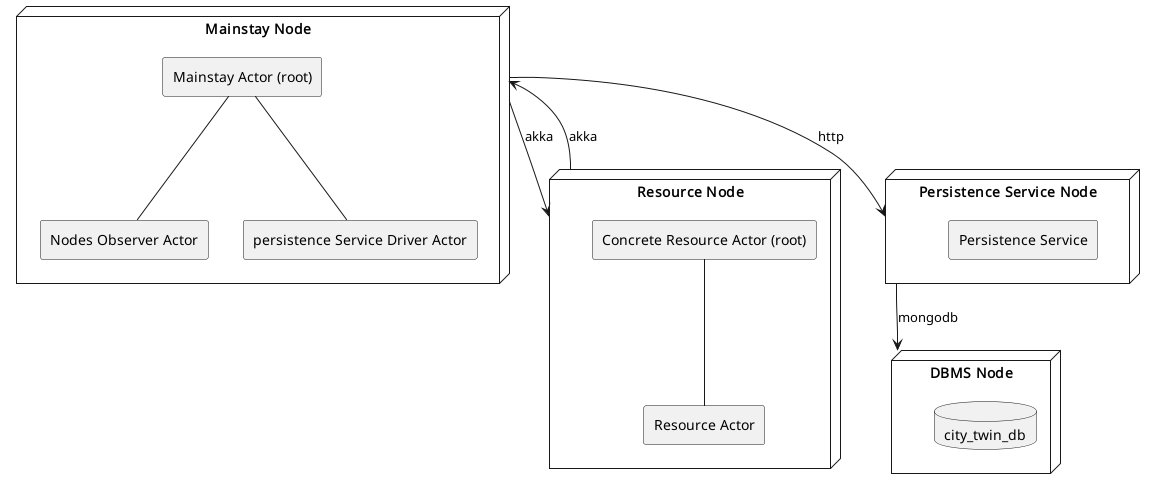
\includegraphics[width=\textwidth]{../assets/images/nodes-component-diagram.png}
    \label{fig:nodes-component-diagram}
\end{figure}

\subsection{Behaviour}

TODO

\subsection{Interazioni dei Componenti}

Il comportamento generale del sistema viene definito sulla base di una serie di interazioni tra i componenti. In particolare, le interazioni possono essere raggruppate per definire un determinato aspetto di tale comportamento.

\subsubsection{Aggiornamento Sullo Stato dei Nodi}

Lo scambio di messaggi tra \textit{Nodes Observer Actor} e \textit{Mainstay Actor} (Figura \ref{fig:core-nodes-state-sequence-diagram}) è volto a mantenere aggiornato quest'ultimo sullo stato generale dei nodi del sistema. Nel momento in cui il \textit{Mainstay Actor} riceve un aggiornamento sui nodi, esso aggiorna il proprio stato e lo comunica al \textit{Persistence Service Driver Actor}, che si occupa di rendere persistenti i dati tramite il servizio di persistenza.

\begin{figure}[h]
    \caption{Diagramma di sequenza per l'aggiornamento sullo stato dei nodi del sistema.}
    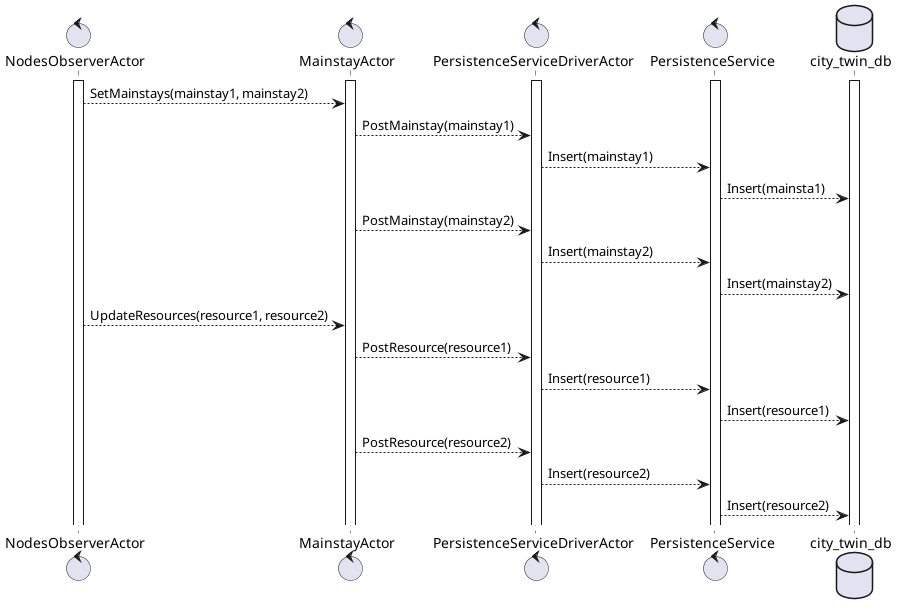
\includegraphics[width=\textwidth]{../assets/images/core-nodes-state-sequence-diagram.png}
    \label{fig:core-nodes-state-sequence-diagram}
\end{figure}

\subsubsection{Aggiornamento Sullo Stato delle Risorse}

Lo scambio di messaggi tra \textit{Resource Actor} e \textit{Mainstay Actor} (Figura \ref{fig:core-resource-state-exchange-sequence-diagram}) è utile a:
\begin{itemize}
    \item Ottenere lo stato delle altre risorse e comunicare il proprio nel caso un cui il nodo \textit{Resource} modella un attuatore.
    \item Comunicare lo stato della risorsa nel caso un cui il nodo \textit{Resource} modella un sensore.
\end{itemize}

In ogni caso, quando il \textit{Mainstay Actor} riceve un aggiornamento, lo comunica al servizio di persistenza tramite il \textit{Persistence Service Driver Actor}.

\begin{figure}[h]
    \caption{Diagramma di sequenza per lo scambio dello stato delle risorse.}
    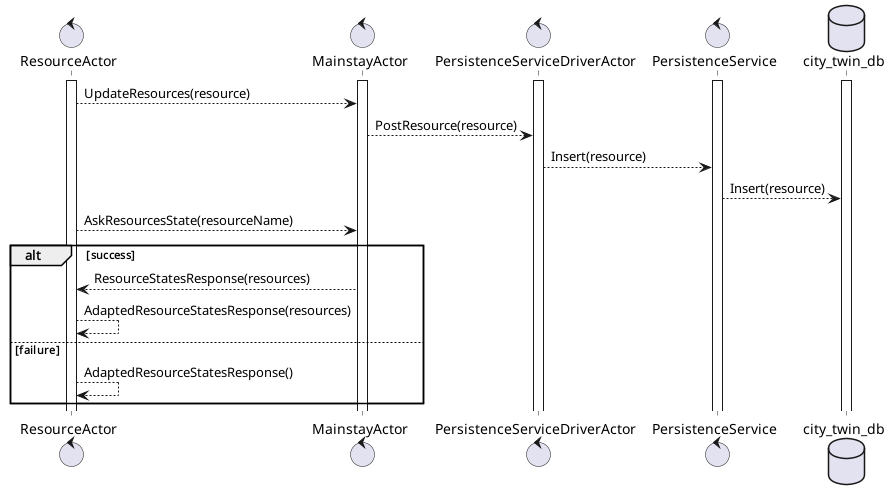
\includegraphics[width=\textwidth]{../assets/images/core-resource-state-exchange-sequence-diagram.png}
    \label{fig:core-resource-state-exchange-sequence-diagram}
\end{figure}

\subsubsection{Sincronizzazione dei Nodi Mainstay}

Come detto precedentemente, i nodi \textit{Mainstay} sono i pilastri portanti dell'intero sistema e si occupano della gestione dei dati riguardanti le risorse e i nodi. I nodi \textit{Mainstay} devono essere sempre sincronizzati tra loro, in modo da poter garantire la coerenza dei dati. Per questo motivo, i nodi \textit{Mainstay} si sincronizzano ogni volta che una risorsa manda il suo stato ad uno di questi. In Figura \ref{fig:core-mainstays-sync-sequence-diagram} viene presentato il diagramma di sequenza per la sincronizzazione dei nodi \textit{Mainstay}.

\begin{figure}[h]
    \caption{Diagramma di sequenza per la sincronizzazione dei nodi Mainstay.}
    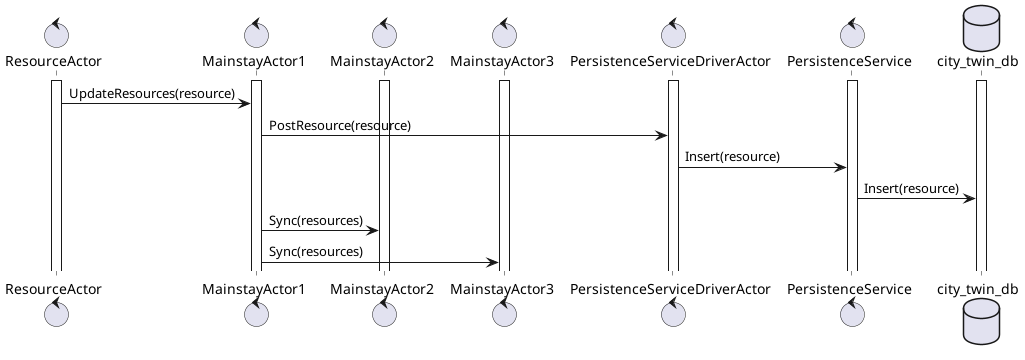
\includegraphics[width=\textwidth]{../assets/images/core-mainstays-sync-sequence-diagram.png}
    \label{fig:core-mainstays-sync-sequence-diagram}
\end{figure}

\subsubsection{Aggiornamento del Pannello di Controllo}

Il comportamento del \textit{Control Panel} (Figura \ref{fig:control-panel-sequence-diagram}) viene modellato come un caso particolare di risorsa che comunica con il \textit{Mainstay Actor} per ottenere lo stato delle risorse e dei nodi. Inoltre, il \textit{Control Panel} comunica con il servizio di persistenza per ottenere lo storico dei dati e calcolare le statistiche.

\begin{figure}[h]
    \caption{Diagramma di sequenza per l'aggiornamento del pannello di controllo.}
    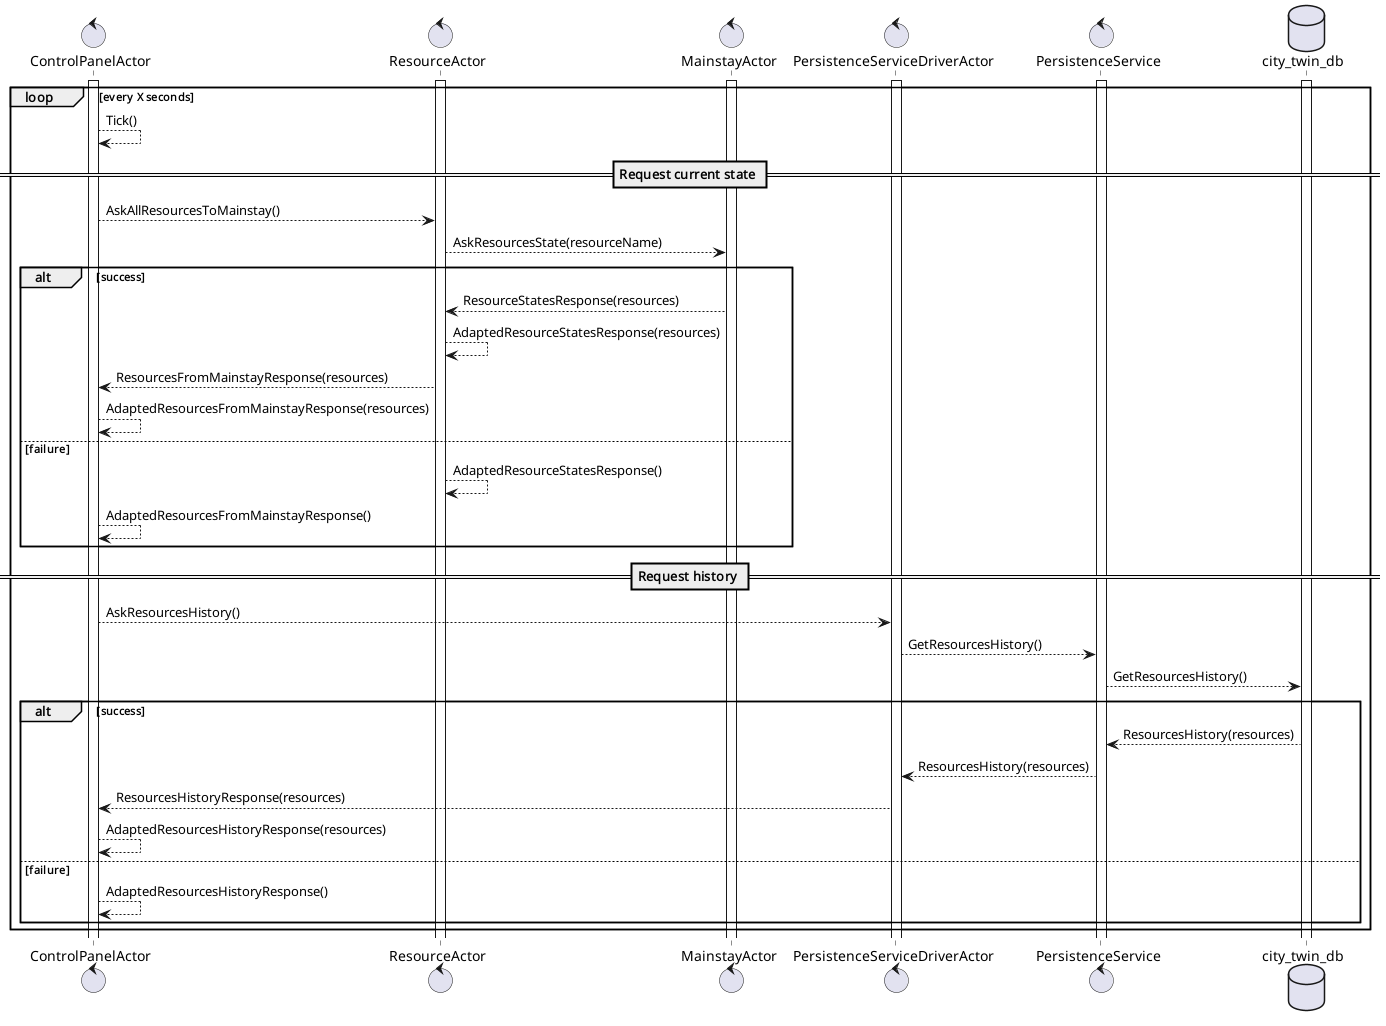
\includegraphics[width=\textwidth]{../assets/images/control-panel-sequence-diagram.png}
    \label{fig:control-panel-sequence-diagram}
\end{figure}

\section{Implementation Details}

Just report interesting / non-trivial / non-obvious implementation details.

This section is expected to be short in case some documentation (e.g. Javadoc or Swagger Spec) has been produced for the software artefacts.
%
This this case, the produced documentation should be referenced here.

\section{Self-assessment / Validation}

Choose a criterion for the evaluation of the produced software and \textbf{its compliance to the requirements above}.

Pseudo-formal or formal criteria are preferred.

In case of a test-driven development, describe tests here and possibly report the amount of passing tests, the total amount of tests and, possibly, the test coverage.

\section{Istruzioni per il Deploy}

%Explain here how to install and launch the produced software artefacts.
%
%Assume the softaware must be installed on a totally virgin environment.
%
%So, report \textbf{any} configuration step.

%Gradle and Docker may be useful here to ensure the deployment and launch processes to be easy.
\subsection{Requisiti in comune}
\begin{itemize}
    \item Scala 3.3.0
    \item Java openjdk 17.0.7
    \item SBT 1.x
    \item Docker
    \item Docker Compose
\end{itemize}

\subsection{Requisiti specifici per piattaforma}
\subsubsection{Linux}
\begin{itemize}
    \item unzip
\end{itemize}

\subsubsection{Windows}
\begin{itemize}
    \item Powershell
    \item tar
\end{itemize}

\section{Avvio del sistema}

%Show how to use the produced software artefacts.

%Ideally, there should be at least one example for each scenario proposed above.

Prima di tutto, avviare il servizio di persistenza:

\begin{lstlisting}[language=bash]
    docker compose build
    docker compose up
\end{lstlisting}
Quindi avviare il resto del sistema in un altro terminale:

Su Linux (bash):

\begin{lstlisting}[language=bash]
    ./scripts/startup.sh
\end{lstlisting}

Su Windows (Powershell):

\begin{lstlisting}[language=bash]
    ./scripts/startup.bat
\end{lstlisting}

\section{Conclusioni}

%Recap what you did
In conclusione possiamo evidenziare come il progetto abbia raggiunto gli obiettivi prefissati, ovvero la realizzazione di un sistema distribuito per il monitoraggio di una Smart City. Il sistema è stato sviluppato in maniera modulare, in modo da poter essere facilmente esteso e mantenuto. Inoltre, il sistema è stato progettato per essere scalabile e resiliente, in modo da poter essere utilizzato in un contesto reale.

\subsection{Sviluppi futuri}

%Recap what you did \emph{not}
Tra i vari miglioramenti a cui abbiamo pensato, i più significativi sono:
\begin{itemize}
    \item Utilizzo di una mappa geografica reale (simile a \textit{Google Maps}): Integrare una mappa geografica reale all'interno del sistema, consentendo di posizionare le risorse virtuali in base alle coordinate reali delle smart city. Questo migliorerebbe la precisione della modellazione e consentirebbe una rappresentazione più accurata dell'ambiente urbano.
    \item Sviluppo delle interfacce grafiche con applicazioni web in modo da renderle accessibili da dispositivi di vario genere (computer, smartphone, tablet, ecc.).;
    \item Possibilità per le risorse di tipo \textit{Act} di accedere allo storico dei dati rendendo trasparente il servizio di persistenza;
    \item Sostituzione dei sensori virtualizzati con sensori reali, in modo da poter effettuare un deployment su larga scala in un contesto reale.
    \item Implementazione di un sistema di autenticazione e autorizzazione per garantire la sicurezza del sistema.
    \item Implementazione di un sistema di notifiche per avvisare gli utenti in caso di eventi critici.
    \item Espansione delle funzionalità di analisi con l'ausilio di sistemi \textit{Big Data}: Introduzione di capacità di analisi avanzate per estrarre insight più profondi dai dati raccolti, ad esempio, analisi predittive per prevedere eventi futuri o rilevare anomalie in tempo reale.
    \item Implementazione di AI e Machine Learning: Integrazione di algoritmi di intelligenza artificiale e machine learning per l'automazione delle decisioni basate sui dati e per migliorare l'efficienza operativa delle smart city.
\end{itemize}

\subsection{What did we learned}

Racap what did you learned

\section*{Stylistic Notes}

Use a uniform style, especially when writing formal stuff: $X$, X, $\mathbf{X}$, $\mathcal{X}$, \texttt{X} are all different symbols possibly referring to different entities.

This is a very short paragraph.

This is a longer paragraph (notice the blank line in the code).
It composed by several sentences.
%
You're invited to use comments within \texttt{.tex} source files to separate sentences composing the same paragraph.

Paragraph should be logically atomic: a subordinate sentence from one paragraph should always refer to another sentence from within the same paragraph.

The first line of a paragraph is usually indented.
%
This is intended: it is the way \LaTeX{} lets the reader know a new paragraph is beginning.

Use the \href{https://en.wikibooks.org/wiki/LaTeX/Source_Code_Listings}{\texttt{listing}} package for inserting scripts into the \LaTeX{} source.

\nocite{*} % Includes all references from the `references.bib` file
\bibliographystyle{plain}
\bibliography{references}

\end{document}
